%%%%%%%%%%%%%%%%%%%%%%%%%%%%%%%%%%%%%%%%%%%%%%%%%%%%%%%%%%%%%%%%%%%%%%%%%%%%%%%%
%2345678901234567890123456789012345678901234567890123456789012345678901234567890
%        1         2         3         4         5         6         7         8

\documentclass[letterpaper, 10 pt, conference]{ieeeconf}  % Comment this line out if you need a4paper

%\documentclass[a4paper, 10pt, conference]{ieeeconf}      % Use this line for a4 paper

\IEEEoverridecommandlockouts                              % This command is only needed if 
                                                          % you want to use the \thanks command

\overrideIEEEmargins                                      % Needed to meet printer requirements.

%In case you encounter the following error:
%Error 1010 The PDF file may be corrupt (unable to open PDF file) OR
%Error 1000 An error occurred while parsing a contents stream. Unable to analyze the PDF file.
%This is a known problem with pdfLaTeX conversion filter. The file cannot be opened with acrobat reader
%Please use one of the alternatives below to circumvent this error by uncommenting one or the other
%\pdfobjcompresslevel=0
%\pdfminorversion=4

% See the \addtolength command later in the file to balance the column lengths
% on the last page of the document

\usepackage{epsfig}
\usepackage{float}
\usepackage{threeparttable}
\usepackage{subfigure}
\usepackage{url}

% The following packages can be found on http:\\www.ctan.org
%\usepackage{graphics} % for pdf, bitmapped graphics files
%\usepackage{epsfig} % for postscript graphics files
%\usepackage{mathptmx} % assumes new font selection scheme installed
%\usepackage{times} % assumes new font selection scheme installed
\usepackage{amsmath} % assumes amsmath package installed
\usepackage{amssymb}  % assumes amsmath package installed

\usepackage{bigstrut,multirow}
	
\usepackage[colorlinks=false, pdfborder={0 0 0}]{hyperref}
\usepackage{cleveref}
\crefname{figure}{fig}{figs}

\usepackage{microtype}


\title{\LARGE \bf
Data-efficient CNN-based Multi-robot Map Building with Panoramic Camera.
}


% \author{ Jincheng Yu$^{1}$,  Zhilin Xu$^{1}$, Feng Gao$^{1}$, Zhaoliang Zhang$^{1}$ and Yu Wang$^{1}$ % <-this % stops a space
% \thanks{*This work was not supported by any organization} % <-this % stops a space
% \thanks{$^{1}$Electronic Engineering Department,
%         Tsinghua University, Beijing, China
%         {\tt\small yjc16@mails.tsinghua.edu.cn, yu-wang@tsinghua.edu.cn}}%
% }


\begin{document}

\maketitle
\thispagestyle{empty}
\pagestyle{empty}


%%%%%%%%%%%%%%%%%%%%%%%%%%%%%%%%%%%%%%%%%%%%%%%%%%%%%%%%%%%%%%%%%%%%%%%%%%%%%%%%
\begin{abstract}
Multi-robot map building of unknown environments is a fundamental problem for multi-robot autonomous robotics. 
Different from single-robot's huge on-board communication bandwidth, the limited communication resources between robots becomes the bottleneck of the multi-robot map building.
In order to do multi-robot map building in communication constrained environments, this paper proposes a data-efficient map representation and merging method based on topology map, called PRET.
% (Place Representor Embedded Topology map)
PRET uses CNN to generate place representor of each new comming place and embeds the representor to the topology map.
Based on the representors, the topology maps of different robots can be easily shared and merged with little communication resources.
Compared with the tranditional grid map. The data transfer is reduced by ?\%. The navigation path is only ?\% higher than the grid map. %结果稍微丰富下
\end{abstract}

\section{Introduction}
\label{sec:intro}

With the development of algorithms and computation platforms, a single moving robot can navigate and build map in a novel environment. 
Limited by the perception range, the system capability of a single robot is not sufficient to deal with tasks in complex environments.
The cooperation of different robots can greatly improve the system capability, and the multi-robot system is a promising research field.

Distributed Simultaneously Localization and Mapping (DSLAM)~\cite{corah2019communication, cieslewski2018data}, which provides the status of different robots and the environment, is a fundamental problem for multi-robot systems, including multi-robot navigation \cite{tanner2005towards} and rescue \cite{baxter2007multi}. As illustrated in \Cref{fig:DSLAMframe}, there are three function thread on each robot, Visual Odometry (VO), Map Building (Map) and Place Recognition (PR). VO reads two time adjacent input images and calculates the relative pose between these images, and finial produces the trajectory of the robots. PR generates compact image representation to produce the candidate place recognition matches between different robots. Map thread records trajectory and builds the environment into local map.

\begin{figure*}[t]
    \begin{minipage}[t]{0.3\linewidth}  
    \centering
    \subfigure[ DSLAM framework. Each frame is fed to VO to calculate trajectory. The local map is build based on the trajectory. Some key frames are fed to PR to encode the scenes into descriptors for inter-robot scene matching. When the same scene is detected with different robots, the local maps of these robots are merged into global map. In this work, we adopt panoramic camera and CNN to DSLAM system. Use topology map for both PR and Map.
    ] {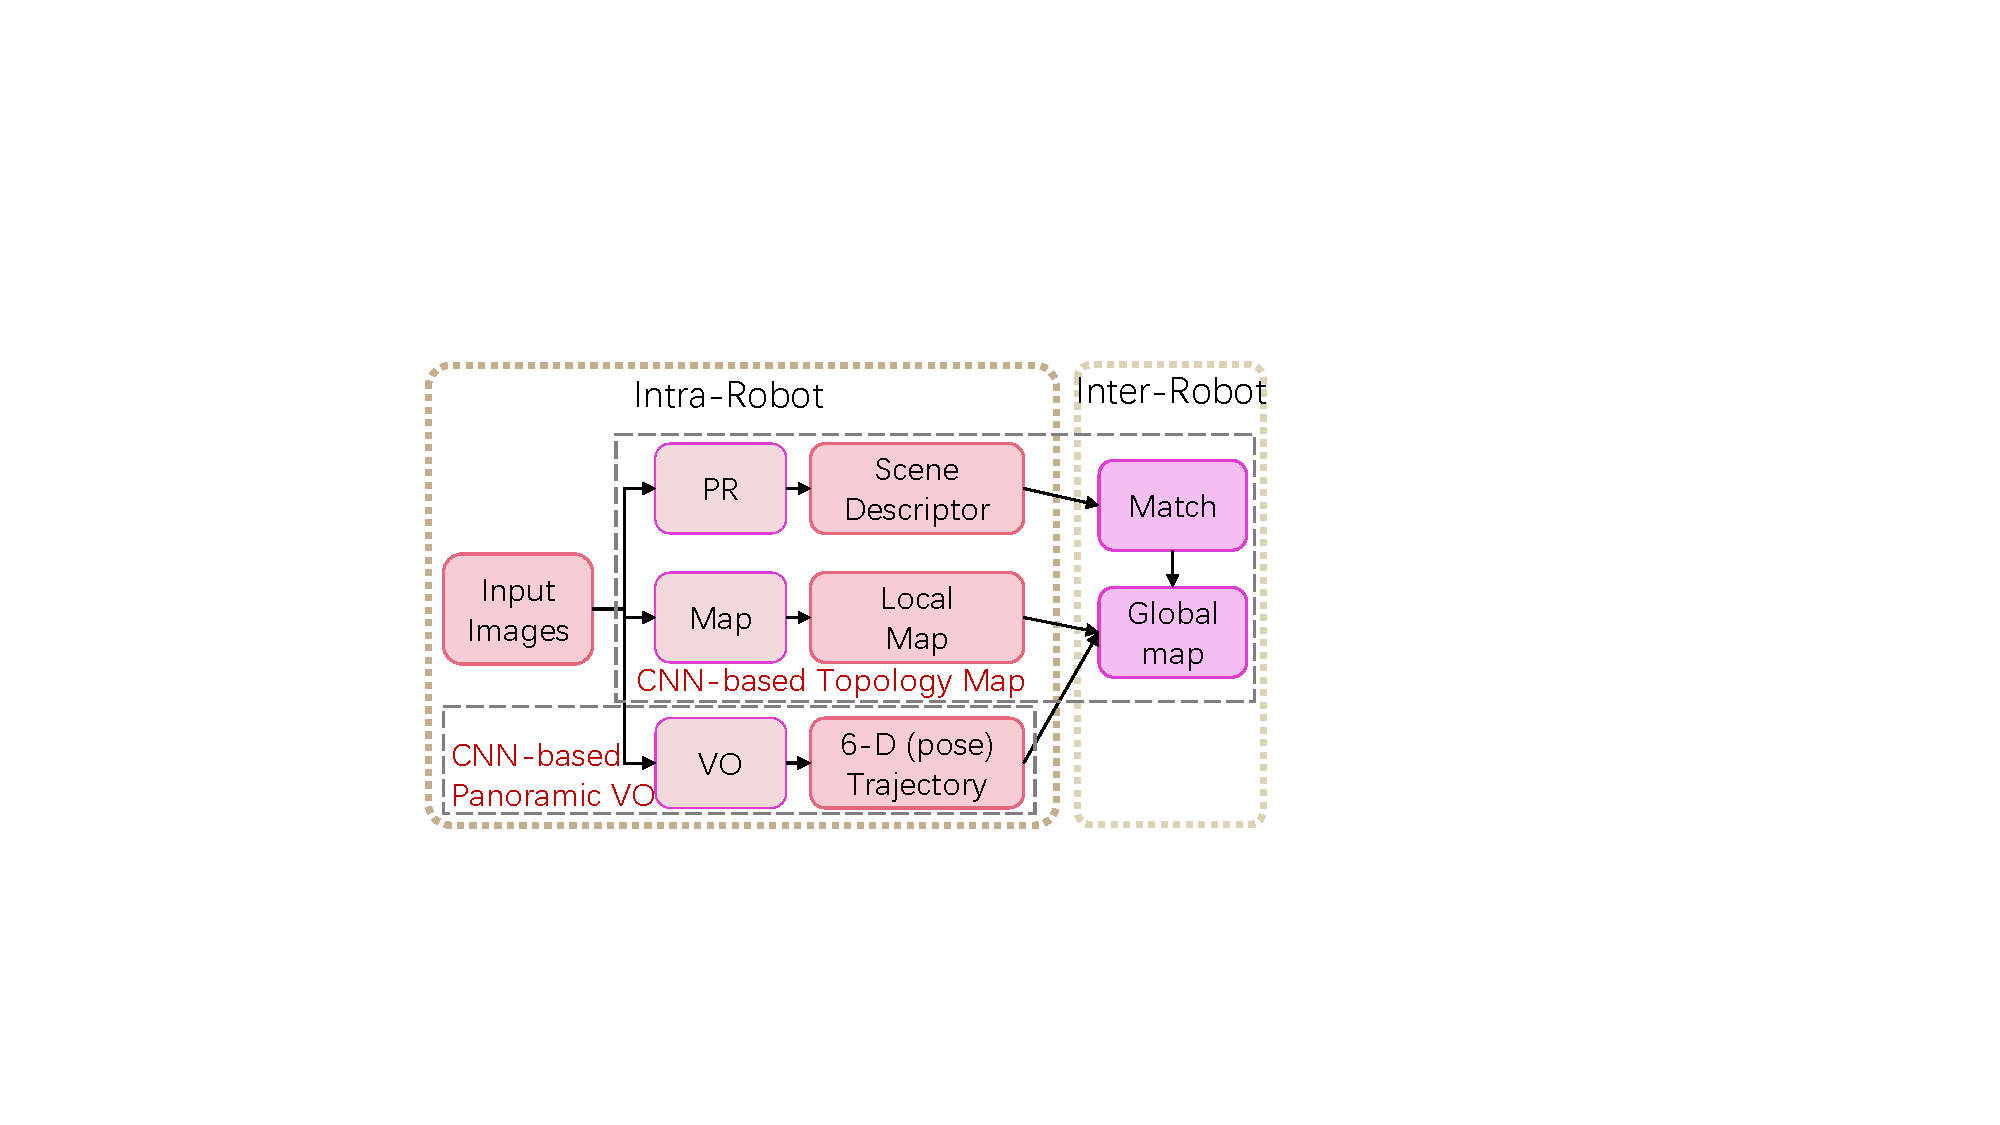
\includegraphics[width=0.95\textwidth]{fig/DSLAMframe.pdf}\label{fig:DSLAMframe}}
    \end{minipage}
    \begin{minipage}[t]{0.7\linewidth}  
    \centering  
    \subfigure[ Our CNN-based DSLAM system with panoramic camera. For VO, we use CNN to calculated the poses between different splited panoramic image frames \textcircled{1} and use graph optimization to fine-tune the camera pose of adjacent time. For Map and PR, we adopt CNN to generate descriptors \textcircled{3} for place recognition and build topology map based on the descriptors \textcircled{4}. We derectly match the topology map between robots \textcircled{5} and merge the local topology map \textcircled{6}.
    ] {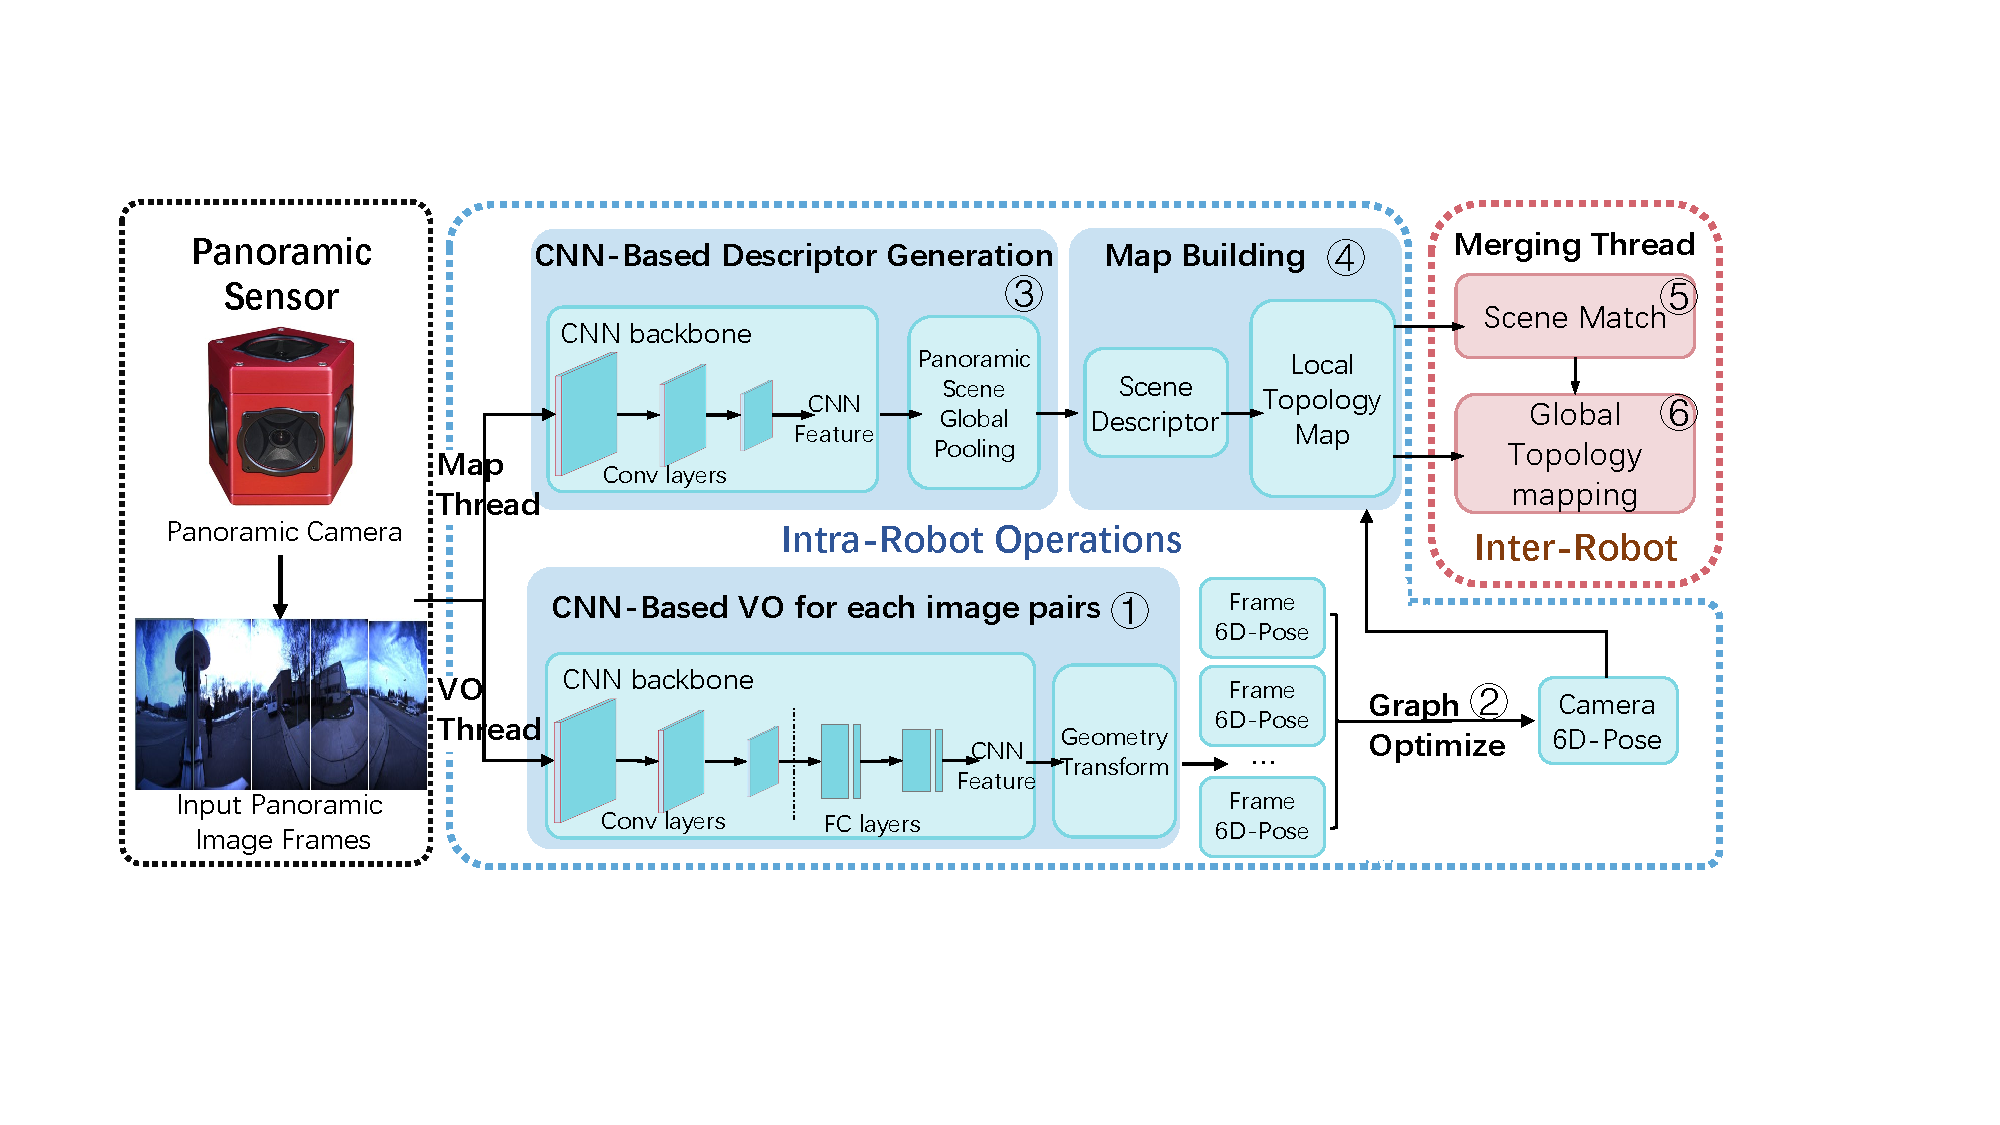
\includegraphics[width=0.95\linewidth]{fig/framework.pdf}\label{fig:framework}} 
    \end{minipage}
    \caption{DSLAM overview. \Cref{fig:DSLAMframe} shows the general DSLAM framework. \Cref{fig:framework} shows our CNN-based method with panoramic camera and topology map.
    }
\label{fig:overview}
\end{figure*}



\section{Related work}
\label{sec:related}

\subsection{Visual Odometry}

Visual Odometry (VO) is crucial for various applications in the multi-robot system, such as Distributed Simultaneously Localization and Mapping (DSLAM)~\cite{corah2019communication, cieslewski2018data}, and multi-robot navigation \cite{tanner2005towards}.
According to the calculation method of pose, current existing VO schemes can be mainly divided into Traditional methods which are usually hand-crafted stage-wise systems, and deep learning-based methods which can infer the pose or the depth from a single image by using Convolutional Neural Network (CNN).
Traditional methods use feature-based methods or direct methods to search for the corresponding points, and multi-view geometry to estimate the pose.
The feature-based methods, like SIFT \cite{Lowe-478} and ORB \cite{Rublee-orb}, search for corresponding keypoints by matching hand-crafted high-dimensional feature descriptors.
The direct methods, such as LSD-SLAM \cite{LSD-SLAM}, directly exploit pixel intensity values to match the corresponding points.

The Traditional methods rely on the depth data of stereo camera \cite{Howard-stereo} or RGB-D \cite{Huang-RGBD} camera to calculate the scale factor of translation.
However, the cost of obtaining deep data is relatively high. Compared to stereo or RGB-d cameras, monocular cameras are more economical and easier to calibrate. 
Recently, some deep learning-based methods have chosen to use monocular data to predict depth and scale. 
Zhou, et al. \cite{zhou2017unsupervised} used unsupervised methods to restore depth and pose from monocular data.
Bian, et al. \cite{bian2019unsupervised} obtained a uniform scale pose through per-pixel-min geometry consistency loss without the depth data of stereo camera or RGB-D camera.

The various VO schemes mentioned above, although their pipeline may be different from each other, have a common premise that there must be sufficient overlap between two adjacent frames.
Only if this condition is met, VO can correctly calculate the relative motion between the two frames.
Monocular cameras, stereo cameras, and RGB-D cameras are all limited Field-of-View (FoV) cameras.
The limited FoV based VO or SLAM systems have four inherent defects:

1) Difficult to handle scenes lacking overlap \cite{ji2020panoramic}.
For a common limited FoV camera, fast movement especially fast rotation will lead to a reduction in the overlap between consecutive frames, resulting in unreliable VO output and even tracking failure. 
This problem can be exacerbated in the SLAM systems that require high-definition maps, where a large format sensor (e.g., $4000 \times 3000$ pixels compared to a commonly used $640 \times 480$ sensor) requires a wide baseline shooting mode because of limited imaging and memory access speed.

2) Difficult to handle movement in dynamic scenes \cite{chen2019palvo}.
In the pipeline of VO, multi-view geometry or CNN methods are used to estimate the pose. 
Both of these methods assume that the robot is in a static scene, since it is unreliable to model landmarks corresponding to dynamic objects  (such as pedestrians, vehicles, etc.). 
However, the actual world is not always static.
Therefore, certain algorithms, such as RANSAC (Random Sample Consensus), are applied to eliminate the effects of dynamic objects in the VO systems.
These algorithms are effective only when the dynamic components are negligible in the entire FoV.
However, it is not surprising that dynamic objects occupy most of the FoV in actual use for a limited FoV camera.
In this case, the pose estimation by the VO system can hardly be kept consistent, and even worse, the VO system may fail to track.

3) Difficult to handle texture-less scenes \cite{hu2019indoor}.
For a limited FoV camera, it’s not strange to encounter situations where texture-less objects occupy most of the FoV in actual use.
For example, if the camera shoots a white wall, most of the image will be occupied by the wall, and there is not enough texture to estimate the motion of the camera.

4) Difficult to deal with Place Recognition (PR) from different view \cite{ji2020panoramic}.
PR generates compact image representation to produce the candidate place recognition matches between different robots.
If two robots pass through the same place from different directions, the scene they see is usually different, and it is difficult for the DSLAM system to match them.
For example, if a robot passes a crossroad and another robot crosses the same crossroad in the opposite or vertical direction, it is difficult for the robots to recognize that they have passed the same crossroad.

In view of this, we propose to apply panoramic camera to the visual odometry in this paper.
Using the panoramic camera can solve or alleviate the four inherent defects mentioned above.
One of the obvious benefits of $360^{\circ}$ panoramas is that it can ensure that there is enough overlap area between adjacent frames despite fast movement and rapid rotation, and it can also solve the problem of Place Recognition from different view.
At the same time, the probability is extremely low that dynamic or texture-less objects occupy most of the FoV in a panoramic camera.
Cubemap-SLAM \cite{wang2018cubemapslam} uses a cubic model to implement a robust and accurate feature-based SLAM for fisheye cameras with large FoV.
PAN-SLAM \cite{ji2020panoramic} adapts to the framework of ORB-SLAM and designs a feature-based panoramic SLAM system.
Deep learning-based VO schemes have advantages in depth prediction \cite{zhou2017unsupervised,bian2019unsupervised}, but there is currently no deep learning-based VO method for panoramic cameras.
Like the stereo datasets and the rgbd datasets, the panoramic datasets are more expensive \cite{chen2019palvo}, while the monocular datasets are more economical and easier to record.
The deep learning-based VO requires a lot of data for training, which is one of the reasons why the current deep learning-based methods are mainly monocular VO.
Jeong, et al. \cite{jeong2013trinocular} modeled the trinocular VO with large FoV as the pose optimization problem of five monocular VOs, but they used the traditional method SIFT.
We propose to divide the panoramic image into multiple monocular images, use deep learning-based monocular VO to calculate multiple sets of poses, and use graph optimization to obtain the final pose.


\bibliographystyle{IEEEtran}
\bibliography{src/fpgaslam}

\end{document}
